\documentclass{tufte-book}
% file: tufte-book-preamble.tex

\hypersetup{colorlinks}% uncomment this line if you prefer colored hyperlinks (e.g., for onscreen viewing)
\usepackage{makeidx}

% If they're installed, use Bergamo and Chantilly from www.fontsite.com.
% They're clones of Bembo and Gill Sans, respectively.
%\IfFileExists{bergamo.sty}{\usepackage[osf]{bergamo}}{}% Bembo
%\IfFileExists{chantill.sty}{\usepackage{chantill}}{}% Gill Sans

%\usepackage{microtype}

%%
% Just some sample text
\usepackage{lipsum}

%%
% For nicely typeset tabular material
\usepackage{booktabs}

%%
% For graphics / images
\usepackage{graphicx}
\setkeys{Gin}{width=\linewidth,totalheight=\textheight,keepaspectratio}
\graphicspath{{graphics/}}

% The fancyvrb package lets us customize the formatting of verbatim
% environments.  We use a slightly smaller font.
\usepackage{fancyvrb}
\fvset{fontsize=\normalsize}

%%
% Prints argument within hanging parentheses (i.e., parentheses that take
% up no horizontal space).  Useful in tabular environments.
\newcommand{\hangp}[1]{\makebox[0pt][r]{(}#1\makebox[0pt][l]{)}}

%%
% Prints an asterisk that takes up no horizontal space.
% Useful in tabular environments.
\newcommand{\hangstar}{\makebox[0pt][l]{*}}

%%
% Prints a trailing space in a smart way.
\usepackage{xspace}

%%
% Some shortcuts for Tufte's book titles.  The lowercase commands will
% produce the initials of the book title in italics.  The all-caps commands
% will print out the full title of the book in italics.
\newcommand{\vdqi}{\textit{VDQI}\xspace}
\newcommand{\ei}{\textit{EI}\xspace}
\newcommand{\ve}{\textit{VE}\xspace}
\newcommand{\be}{\textit{BE}\xspace}
\newcommand{\VDQI}{\textit{The Visual Display of Quantitative Information}\xspace}
\newcommand{\EI}{\textit{Envisioning Information}\xspace}
\newcommand{\VE}{\textit{Visual Explanations}\xspace}
\newcommand{\BE}{\textit{Beautiful Evidence}\xspace}

\newcommand{\TL}{Tufte-\LaTeX\xspace}

% Prints the month name (e.g., January) and the year (e.g., 2008)
\newcommand{\monthyear}{%
  \ifcase\month\or January\or February\or March\or April\or May\or June\or
  July\or August\or September\or October\or November\or
  December\fi\space\number\year
}


% Prints an epigraph and speaker in sans serif, all-caps type.
\newcommand{\openepigraph}[2]{%
  %\sffamily\fontsize{14}{16}\selectfont
  \begin{fullwidth}
  \sffamily\large
  \begin{doublespace}
  \noindent\allcaps{#1}\\% epigraph
  \noindent\allcaps{#2}% author
  \end{doublespace}
  \end{fullwidth}
}

% Inserts a blank page
\newcommand{\blankpage}{\newpage\hbox{}\thispagestyle{empty}\newpage}

\usepackage{units}

% Typesets the font size, leading, and measure in the form of 10/12x26 pc.
\newcommand{\measure}[3]{#1/#2$\times$\unit[#3]{pc}}

% Macros for typesetting the documentation
\newcommand{\hlred}[1]{\textcolor{Maroon}{#1}}% prints in red
\newcommand{\hangleft}[1]{\makebox[0pt][r]{#1}}
\newcommand{\hairsp}{\hspace{1pt}}% hair space
\newcommand{\hquad}{\hskip0.5em\relax}% half quad space
\newcommand{\TODO}{\textcolor{red}{\bf TODO!}\xspace}
\newcommand{\ie}{\textit{i.\hairsp{}e.}\xspace}
\newcommand{\eg}{\textit{e.\hairsp{}g.}\xspace}
\newcommand{\na}{\quad--}% used in tables for N/A cells
\providecommand{\XeLaTeX}{X\lower.5ex\hbox{\kern-0.15em\reflectbox{E}}\kern-0.1em\LaTeX}
\newcommand{\tXeLaTeX}{\XeLaTeX\index{XeLaTeX@\protect\XeLaTeX}}
% \index{\texttt{\textbackslash xyz}@\hangleft{\texttt{\textbackslash}}\texttt{xyz}}
\newcommand{\tuftebs}{\symbol{'134}}% a backslash in tt type in OT1/T1
\newcommand{\doccmdnoindex}[2][]{\texttt{\tuftebs#2}}% command name -- adds backslash automatically (and doesn't add cmd to the index)
\newcommand{\doccmddef}[2][]{%
  \hlred{\texttt{\tuftebs#2}}\label{cmd:#2}%
  \ifthenelse{\isempty{#1}}%
    {% add the command to the index
      \index{#2 command@\protect\hangleft{\texttt{\tuftebs}}\texttt{#2}}% command name
    }%
    {% add the command and package to the index
      \index{#2 command@\protect\hangleft{\texttt{\tuftebs}}\texttt{#2} (\texttt{#1} package)}% command name
      \index{#1 package@\texttt{#1} package}\index{packages!#1@\texttt{#1}}% package name
    }%
}% command name -- adds backslash automatically
\newcommand{\doccmd}[2][]{%
  \texttt{\tuftebs#2}%
  \ifthenelse{\isempty{#1}}%
    {% add the command to the index
      \index{#2 command@\protect\hangleft{\texttt{\tuftebs}}\texttt{#2}}% command name
    }%
    {% add the command and package to the index
      \index{#2 command@\protect\hangleft{\texttt{\tuftebs}}\texttt{#2} (\texttt{#1} package)}% command name
      \index{#1 package@\texttt{#1} package}\index{packages!#1@\texttt{#1}}% package name
    }%
}% command name -- adds backslash automatically
\newcommand{\docopt}[1]{\ensuremath{\langle}\textrm{\textit{#1}}\ensuremath{\rangle}}% optional command argument
\newcommand{\docarg}[1]{\textrm{\textit{#1}}}% (required) command argument
\newenvironment{docspec}{\begin{quotation}\ttfamily\parskip0pt\parindent0pt\ignorespaces}{\end{quotation}}% command specification environment
\newcommand{\docenv}[1]{\texttt{#1}\index{#1 environment@\texttt{#1} environment}\index{environments!#1@\texttt{#1}}}% environment name
\newcommand{\docenvdef}[1]{\hlred{\texttt{#1}}\label{env:#1}\index{#1 environment@\texttt{#1} environment}\index{environments!#1@\texttt{#1}}}% environment name
\newcommand{\docpkg}[1]{\texttt{#1}\index{#1 package@\texttt{#1} package}\index{packages!#1@\texttt{#1}}}% package name
\newcommand{\doccls}[1]{\texttt{#1}}% document class name
\newcommand{\docclsopt}[1]{\texttt{#1}\index{#1 class option@\texttt{#1} class option}\index{class options!#1@\texttt{#1}}}% document class option name
\newcommand{\docclsoptdef}[1]{\hlred{\texttt{#1}}\label{clsopt:#1}\index{#1 class option@\texttt{#1} class option}\index{class options!#1@\texttt{#1}}}% document class option name defined
\newcommand{\docmsg}[2]{\bigskip\begin{fullwidth}\noindent\ttfamily#1\end{fullwidth}\medskip\par\noindent#2}
\newcommand{\docfilehook}[2]{\texttt{#1}\index{file hooks!#2}\index{#1@\texttt{#1}}}
\newcommand{\doccounter}[1]{\texttt{#1}\index{#1 counter@\texttt{#1} counter}}

% file: pseudo-preamble.tex

% math
\usepackage{amsmath}
\newcommand{\set}[1]{\{#1\}}

% algorithm
\usepackage{algorithm}
\usepackage[noend]{algpseudocode}
\newcommand{\hStatex}[0]{\vspace{5pt}}

% color
\newcommand{\teal}[1]{\textcolor{teal}{#1}}


\title{Collection of Algorithms Pseudocode}
\author[hengxin]{Hengfeng Wei}
\publisher{Ant}

\makeindex

\begin{document}

\frontmatter

% r.1 blank page
\blankpage

% v.2 epigraphs
\newpage\thispagestyle{empty}
\openepigraph{%
The public is more familiar with bad design than good design.
It is, in effect, conditioned to prefer bad design, 
because that is what it lives with. 
The new becomes threatening, the old reassuring.
}{Paul Rand%, {\itshape Design, Form, and Chaos}
}
\vfill
\openepigraph{%
A designer knows that he has achieved perfection 
not when there is nothing left to add, 
but when there is nothing left to take away.
}{Antoine de Saint-Exup\'{e}ry}
\vfill
\openepigraph{%
\ldots the designer of a new system must not only be the implementor and the first 
large-scale user; the designer should also write the first user manual\ldots 
If I had not participated fully in all these activities, 
literally hundreds of improvements would never have been made, 
because I would never have thought of them or perceived 
why they were important.
}{Donald E. Knuth}


% r.3 full title page
\maketitle

% v.4 copyright page
\newpage
\begin{fullwidth}
~\vfill
\thispagestyle{empty}
\setlength{\parindent}{0pt}
\setlength{\parskip}{\baselineskip}
Copyright \copyright\ \the\year\ \thanklessauthor

\par\smallcaps{Published by \thanklesspublisher}

\par\smallcaps{tufte-latex.googlecode.com}

\par Licensed under the Apache License, Version 2.0 (the ``License''); you may not
use this file except in compliance with the License. You may obtain a copy
of the License at \url{http://www.apache.org/licenses/LICENSE-2.0}. Unless
required by applicable law or agreed to in writing, software distributed
under the License is distributed on an \smallcaps{``AS IS'' BASIS, WITHOUT
WARRANTIES OR CONDITIONS OF ANY KIND}, either express or implied. See the
License for the specific language governing permissions and limitations
under the License.\index{license}

\par\textit{First printing, \monthyear}
\end{fullwidth}

% r.5 contents
\tableofcontents

\listoffigures

\listoftables

% r.7 dedication
\cleardoublepage
~\vfill
\begin{doublespace}
\noindent\fontsize{18}{22}\selectfont\itshape
\nohyphenation
Dedicated to those who appreciate \LaTeX{} 
and the work of \mbox{Edward R.~Tufte} 
and \mbox{Donald E.~Knuth}.
\end{doublespace}
\vfill
\vfill

% r.9 introduction
\cleardoublepage
\chapter*{Introduction}

This is a collection of psuedocode for classic algorithms.

\mainmatter

% file: chapters/iteration-recursion.tex

\chapter{Basic Iterative and Recursive Algorithms}	\label{chapter:iteration-recursion}

% file: algs/horner-rule.tex

\begin{algorithm}[H]
  \caption{Horner rule for polynomial evaluation.}
  \begin{algorithmic}[1]
    \Procedure{Horner}{$A[0 \dots n], x$} \Comment{$A: \set{a_0 \dots a_n}$}
      \State $p \gets A[n]$

      \hStatex
      \For{$i \gets n-1 \;\text{\bf downto } 0$}
	\State $p \gets px + A[i]$
      \EndFor

      \hStatex
      \State \Return $p$
    \EndProcedure
  \end{algorithmic}
\end{algorithm}
% file: algs/integer-mult.tex

\begin{algorithm}[H]
  \caption{Integer Multiplication.}
  \begin{algorithmic}[1]
    \Procedure{Int-Mult}{$y, z$}  \Comment{$y,z \ge 0; \; y, z \in \mathbb{Z}$}
      \If{$z = 0$}
        \State \Return 0
      \EndIf

      \State \Return $\Call{Int-Mult}{cy, \lfloor \frac{z}{c} \rfloor} + y (z \bmod c)$
    \EndProcedure
  \end{algorithmic}
\end{algorithm}

% chapters/sorting.tex

\chapter{Sorting}	\label{chapter:sorting}

% 3-element sorting
\begin{figure}
  \centering
  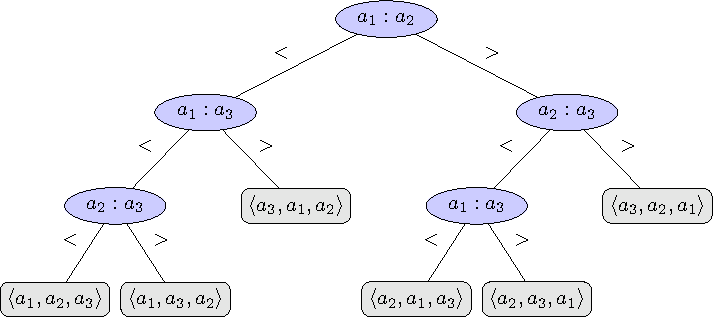
\includegraphics[width = 0.70\textwidth]{figs/3-sorting}
  \caption{$3$-element sorting algorithm represented by a decision tree.}
  \label{fig:3-sorting}
\end{figure}

% file: algs/bubblesort-smallest.tex

\begin{algorithm}[H]
  \caption{Bubblesort (Bubble the smallest element each time.).}
  \label{alg:bubblesort-smallest}
  \begin{algorithmic}[1]
    \Procedure{Bubblesort}{$A[1 \cdots n]$}
      \For{$i \gets 1 \;\text{\bf to } n-1$}
	\For{$j \gets n \;\text{\bf downto } i+1$}
	  \If{$A[j] < A[j-1]$}
	    \State $\Call{Swap}{A[j], A[j-1]}$
	  \EndIf
	\EndFor
      \EndFor
    \EndProcedure
  \end{algorithmic}
\end{algorithm}

% file: algs/bubblesort-largest.tex

\begin{algorithm}[H]
  \caption{Bubblesort (Bubble the largest element each time.).}
  \label{alg:bubblesort-largest}
  \begin{algorithmic}[1]
    \Procedure{Bubblesort}{$A[1 \cdots n]$}
      \For{$i \gets n \;\text{\bf downto } 2$}
	\For{$j \gets 1 \;\text{\bf to } i-1$}
	  \If{$A[j] > A[j+1]$}
	    \State $\Call{Swap}{A[j], A[j+1]}$
	  \EndIf
	\EndFor
      \EndFor
    \EndProcedure
  \end{algorithmic}
\end{algorithm}

% file: algs/bubblesort-improved.tex

\begin{algorithm}[H]
  \caption{Bubblesort (An improved version; from wiki).}
  \label{alg:bubblesort-imporoved}
  \begin{algorithmic}[1]
    \Procedure{Bubblesort}{$A[1 \cdots n]$}
      \Repeat
	\State $newn \gets 0$
	\For{$i \gets 1 \;\text{\bf to } n-1$}
	  \If{$A[i-1] > A[i]$}
	    \State $\Call{Swap}{A[i-1], A[i]}$
	    \State $newn \gets i$
	  \EndIf
	\EndFor
	\State $n \gets newn$
      \Until{$n = 0$}
    \EndProcedure
  \end{algorithmic}
\end{algorithm}


\section{Quicksort}

\textsc{Hoare-Partition} (alg4)
% file: algs/sorting/hoare-partition.tex

\begin{algorithm}[H]
  \caption{Hoare partition.}
  \begin{algorithmic}[]
    \Procedure{Hoare-Partition}{$A, l, r$}
      \State $x \gets A[l]$
      \State $i \gets l$
      \State $j \gets r + 1$

      \Statex
      \While{TRUE}
	\While{$A[++i] < x$}
	  \If{$i = r$}
	    \State \textbf{break}
	  \EndIf
	\EndWhile

	\While{$A[--j] > x$}
	  \If{$j = l$}
	    \State \textbf{break}
	  \EndIf
	\EndWhile

	\Statex
	\If{$i < j$}
	  \State \Call{Swap}{$A, i, j$}
	\EndIf
      \EndWhile

      \Statex
      \State \Call{Swap}{$A, l, j$}
    \EndProcedure
  \end{algorithmic}
\end{algorithm}


\section{Linear Time Sorting}
% file: algs/sorting/selection-sort.tex

\begin{algorithm}[H]
  \caption{Selection Sort.}
  \label{alg:selection-sort}
  \begin{algorithmic}[1]
    \Procedure{Selection-Sort}{$A, n$}
      \For{$i \gets 1 \;\textbf{to}\; n-1$}
	\For{$j \gets i+1 \;\textbf{to}\; n$}
	  \If{$A[j] < A[i]$}
	    \State \Call{Swap}{$A[j], A[i]$}
	  \EndIf
	\EndFor
      \EndFor
    \EndProcedure
  \end{algorithmic}
\end{algorithm}

% file: algs/sorting/counting-sort-cycle.tex

\begin{algorithm}[H]
  \caption{\textsc{Counting-Sort} in place in $O(n + k)$ time.}
  \label{alg:counting-sort}
  \begin{algorithmic}[1]
    \Procedure{Counting-Sort}{$A, k$}
      \State TODO
    \EndProcedure
  \end{algorithmic}
\end{algorithm}


% file: chapters/selection.tex

\chapter{Selection}	\label{chapter:selection}

% 3-element median selection
\begin{figure}
  \centering
  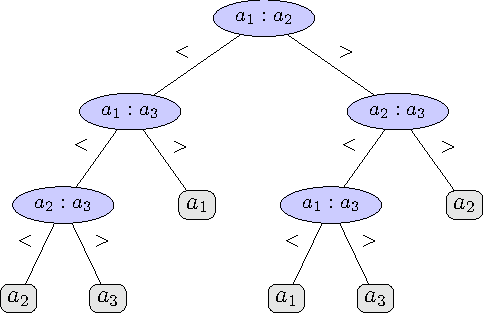
\includegraphics[width = 0.70\textwidth]{figs/3-median}
  \caption{$3$-element median selection algorithm represented by a decision tree.}
  \label{fig:3-median}
\end{figure}

% chapters/dp.tex

\chapter{Dynamic Programming}	\label{chapter:dp}

% file: algs/dp/binom-recursive.tex

\begin{algorithm}[H]
  \caption{Computing $\binom{n}{k}$.}
  \label{alg:binom-recursive}
  \begin{algorithmic}[1]
    \Procedure{Binom}{$n, k$} \Comment{Required: $n \ge k \ge 0$}
      \If{$k = 0 \lor n = k$}
	\State \Return 1
      \EndIf

      \State \Return $\Call{Binom}{n-1, k} + \Call{Binom}{n-1, k-1}$
    \EndProcedure
  \end{algorithmic}
\end{algorithm}


% file: algs/dp/binom-dp.tex

\begin{algorithm}[H]
  \caption{Computing $\binom{n}{k}$ by dynamic programming.}
  \begin{algorithmic}[1]
    \Procedure{Binom}{$n, k$} \Comment{Required: $n \ge k \ge 0$}
      \For{$i \gets 0 \;\text{\bf to}\; n-k$}
	\State $B[i][0] \gets 1$
      \EndFor

      \For{$i \gets 1 \;\text{\bf to}\; k$}
	\State $B[i][i] \gets 1$
      \EndFor

      \For{$j \gets 1 \;\text{\bf to}\; k$}
	\For{$d \gets 1 \;\text{\bf to}\; n-k$}
	  \State $i \gets j + d$
	  \State $B[i][j] \gets B[i-1][j] + B[i-1][j-1]$
	\EndFor
      \EndFor
      \State \Return $B[n][k]$
    \EndProcedure
  \end{algorithmic}
\end{algorithm}



% chapters/tree-traversal.tex

\chapter{Traversal on Trees}	\label{chapter:tree-traversal}

% chapters/tree-dfs.tex

\section{DFS on Trees}	\label{section:tree-dfs}

% file: algs/tree-traversal/dfs/dfs-print-recursive.tex

\begin{algorithm}[H]
  \caption{Recursive DFS pre-order traversal on binary tree.}
  \begin{algorithmic}[]
    \Procedure{Recursive-DFS}{$t$}
      \State print $t.key$

      \Statex
      \If{$t.left \neq \textsf{NIL}$}
	\State \Call{Recursive-DFS}{$t.left$}
      \EndIf
      
      \If{$t.right \neq \textsf{NIL}$}
	\State \Call{Recursive-DFS}{$t.right$}
      \EndIf
    \EndProcedure

    \Statex
    \State \Call{Recursive-DFS}{$T.root$}
  \end{algorithmic}
\end{algorithm}

% file: algs/tree-traversal/dfs/dfs-print-nonrecursive.tex

\begin{algorithm}[H]
  \caption{Iterative DFS pre-order traversal on binary tree.}
  \begin{algorithmic}[]
    \Procedure{Iterative-DFS}{$t$}
      \State $S.\Call{Push}{t}$ \Comment{$S:$ stack}

      \Statex
      \While{$S \neq \emptyset$}
	\State $v \gets S.\Call{Pop}{\null}$
	\State print $v.key$

	\Statex
	\If{$v.right \neq \textsf{NIL}$}
	  \State $S.\Call{Push}{v.right}$
	\EndIf

	\If{$v.left \neq \textsf{NIL}$}
	  \State $S.\Call{Push}{v.left}$
	\EndIf
      \EndWhile
    \EndProcedure

    \Statex
    \State \Call{Iterative-DFS}{$T.root$}
  \end{algorithmic}
\end{algorithm}

% file: algs/tree-traversal/dfs/LCRS-rooted-tree-traversal.tex

\begin{algorithm}[H]
  \caption{Recursive DFS traversal on a rooted tree stored using the ``left-child, right-sibling'' representation.}
  \begin{algorithmic}[]
    \Procedure{Recursive-DFS}{$t$}
      \State print $t.key$

      \Statex
      \If{$t.left\text{-}child \neq \textsf{NIL}$}
	\State \Call{Recursive-DFS}{$t.left\text{-}child$}
      \EndIf
      
      \If{$t.right\text{-}sibling \neq \textsf{NIL}$}
	\State \Call{Recursive-DFS}{$t.right\text{-}sibling$}
      \EndIf
    \EndProcedure

    \Statex
    \State \Call{Recursive-DFS}{$T.root$}
  \end{algorithmic}
\end{algorithm}


% file: algs/sum-of-depths.tex
% for UD Problem 4.2 (a)

\begin{algorithm}[H]
  \caption{Calculate the sum of depths of all nodes of a tree $T$.}
  \label{alg:sum-of-depths}
  \begin{algorithmic}[1]
    \Procedure{Sum-of-Depths}{\null}
      \State \Return $\Call{Sum-of-Depths}{T, 0}$ 
    \EndProcedure

    \Statex
    \Procedure{Sum-of-Depths}{$r, depth$} \Comment{$r$: root of a tree}
      \If{$r$ is a leaf}
        \State \Return $depth$
      \EndIf

      \hStatex
      \State $sum \gets depth$
      \ForAll{child vertex $v$ of $r$}
	\State $sum \gets sum + \Call{Sum-of-Depths}{v, depth + 1}$
      \EndFor
      \State \Return $sum$
    \EndProcedure
  \end{algorithmic}
\end{algorithm}
% file: algs/nodes-at-depth-K.tex
% for UD Problem 4.2 (b)

\begin{algorithm}[H]
  \caption{Count the number of nodes in $T$ at depth $K$.}
  \label{alg:nodes-at-depth-K}
  \begin{algorithmic}[1]
    \Procedure{Nodes-at-Depth}{\null}
      \State \Return $\Call{Nodes-at-Depth}{T, K}$ 
    \EndProcedure

    \Statex
    \Procedure{Nodes-at-Depth}{$r, k$} \Comment{$r$: root of a tree}
      \If{$k = 0$}
        \State \Return 1
      \EndIf

      \hStatex
      \If{$r$ is a leaf}
	\State \Return 0
      \EndIf

      \hStatex
      \State $num \gets 0$
      \ForAll{child vertex $v$ of $r$}
	\State $num \gets num + \Call{Nodes-at-Depth}{v, k - 1}$
      \EndFor
      \State \Return $num$
    \EndProcedure
  \end{algorithmic}
\end{algorithm}

% file: algs/leaf-at-even-depth.tex
% for UD Problem 4.2 (c)

\begin{algorithm}[H]
  \caption{Check whether a tree $T$ has any leaf at an even depth.}
  \label{alg:leaf-at-even-depth}
  \begin{algorithmic}[1]
    \Procedure{Leaf-at-Even-Depth}{\null}
      \State \Return $\Call{Leaf-at-Depth}{T, even = 0}$
    \EndProcedure

    \Statex
    \Procedure{Leaf-at-Depth}{$r, parity$} \Comment{$r$: root of a tree}
      \If{$r$ is a leaf}
        \State \Return $1-parity$
      \EndIf

      \hStatex
      \State $result \gets 0$
      \ForAll{child vertex $v$ of $r$}
	\State $result \gets result \lor \Call{Leaf-at-Depth}{v, 1-parity}$
      \EndFor
      \State \Return $result$
    \EndProcedure
  \end{algorithmic}
\end{algorithm}




% chapters/tree-bfs.tex

\section{BFS on Trees}	\label{section:tree-bfs}

% file: algs/sum-at-depth.tex
% for UD Problem 4.3 (a)

\begin{algorithm}[H]
  \caption{Calculate the sum of contents of nodes of a tree $T$ at each depth.}
  \label{alg:sum-at-depth}
  \begin{algorithmic}[1]
    \Procedure{Sum-at-Depth}{$r$} \Comment{$r$: root of the tree $T$}
      \State \teal{$r.depth \gets 0$}

      \hStatex
      \State $Q \gets \emptyset$
      \State $\Call{Enqueue}{Q, r}$

      \hStatex
      \While{$Q \neq \emptyset$}
	\State $u \gets \Call{Dequeue}{Q}$
	\State \teal{$sumAtDepth[u.depth] \text{\;+=\;} u.content$}

	\hStatex
	\ForAll{child vertex $v$ of $u$}
	  \State \teal{$v.depth \gets u.depth + 1$}
	  \State $\Call{Enqueue}{Q, v}$
	\EndFor
      \EndWhile
    \EndProcedure
  \end{algorithmic}
\end{algorithm}

% file: algs/nodes-at-depth.tex
% for UD Problem 4.3 (b)

\begin{algorithm}[H]
  \caption{Count the number of nodes of a tree $T$ at each depth.}
  \label{alg:nodes-at-depth}
  \begin{algorithmic}[1]
    \Procedure{Nodes-at-Depth}{$r$} \Comment{$r$: root of the tree $T$}
      \State $r.depth \gets 0$

      \hStatex
      \State $Q \gets \emptyset$
      \State $\Call{Enqueue}{Q, r}$

      \hStatex
      \While{$Q \neq \emptyset$}
	\State $u \gets \Call{Dequeue}{Q}$
	\State $nodesAtDepth[u.depth] \text{\;+=\;} 1$

	\hStatex
	\ForAll{child vertex $v$ of $u$}
	  \State $v.depth \gets u.depth + 1$
	  \State $\Call{Enqueue}{Q, v}$
	\EndFor
      \EndWhile

      \hStatex
      \State \Return $\text{argmax}_{K} nodesAtDepth[k]$
    \EndProcedure
  \end{algorithmic}
\end{algorithm}




\backmatter

\bibliography{pseudo}
\bibliographystyle{plainnat}

% \printindex

\end{document}